\documentclass[final,t]{beamer}
\mode<presentation>
  {
  \usetheme{Rochester}
  }
\setbeamertemplate{navigation symbols}{}
\setbeamertemplate{caption}[numbered]
\setbeamertemplate{bibliography item}{\insertbiblabel}

\usepackage{etoolbox}% http://ctan.org/pkg/etoolbox
\apptocmd{\thebibliography}{\scriptsize}{}{}

\usepackage[orientation=portrait,size=a0,scale=1.4,debug]{beamerposter}
\usepackage{lipsum} % for dummy text
\usepackage{graphicx} % for dummy image
\usepackage{tikz} % for tikzpicture
\usepackage{pgfplots} % for plot
\usepackage{ragged2e}
\let\olditem\item
\renewcommand\item{\olditem\justifying}
\usetikzlibrary{arrows,shapes,positioning}
\usepackage[justification=justified]{caption}

\title[]{ \huge Numerical simulations of cryolava flows at the surface of Titan}
\author[]{\Large \textbf{Bastien Bodin}$^1$ \and Daniel Cordier$^1$}
\institute[]{\small $^1$ Groupe de Spectrométrie Moléculaire et Atmosphérique, CNRS -- UMR 7331, Université de Reims Champagne-Ardenne\\ \texttt{bastien.bodin@univ-reims.fr}}
\date{}

\begin{document}

\begin{frame}
\begin{minipage}{0.15\textwidth}
	\includegraphics[height=70mm]{Logos/logo_gsma.png}
\end{minipage}
\begin{minipage}{0.69\textwidth}
	\maketitle
\end{minipage}
\begin{minipage}{0.15\textwidth}
	\includegraphics[height=70mm]{Logos/logo_urca.png}
\end{minipage}

%\vspace{-1cm}

\begin{block}{\textbf{Introduction}}
	\rightskip=0pt\leftskip=0pt
	
	Titan, Saturn's main satellite, is a unique object in the Solar System. This moon has a dense atmosphere, that harbors a complex organic chemistry, and a liquid water ocean under its surface. These features raise major questions such as the possible interaction between the liquid water and the organic matter present on the surface.
	
A possible mechanism for these interior-surface interactions could be cryovolcanism, whose existence is suggested by the presence of $^{40}Ar$ in the atmosphere \cite{nixon}. Some candidate cryovolcanoes have been detected, and the observation of cryolavas would allow us to constrain their physico-chemical properties.

In order to investigate cryolava characteristics, we are developping a numerical model based on the "Smoothed-Particle Hydrodynamics" (SPH) method. The aim of this work is to validate our approach by comparing it with an already published model of cryolava at rest. %Validation du modèle à partir de Davies et al 2010
\end{block}

\vspace{-1cm }

\begin{columns}[t]

  \begin{column}{.495\linewidth}


  
  \begin{block}{\textbf{1. Volcanism in the Solar System}}\rightskip=0pt\leftskip=0pt
  \begin{columns}
  \begin{column}{0.495\textwidth}\rightskip=0pt\leftskip=0pt
  \begin{figure}
  	\centering
  	\includegraphics[scale=0.4]{Fig-Lopes-Dim-2013.png} 
  \end{figure}
  \end{column}
  \begin{column}{0.495\textwidth}\rightskip=0pt\leftskip=0pt
  Multiple objects are subject to volcanism in the Solar System: e.g. Earth, Io, Enceladus or even Titan.
  Two types of physical processes are known to possibly produce "cryolava" on Titan:
  \begin{itemize}
  	\item Impact crater formations (e.g. Selk, \cite{Neish})
  	\item Cryovolcanoes (some candidates, fig. \ref{fig:MohiniFluctus})
  \end{itemize}
  
  ~
  
  \begin{figure}
  	\caption{(a) SAR and VIMS data for the Sotra Patera region. (b, c, d) Results of SAR stereo over the Sotra region. (b) SAR. (c) Color-coded DTM. (d) Merged SAR and DTM. (e) Scale comparison between Mohini Fluctus and the Great Lakes. Adapted from \emph{Lopes et al. (2013)} \cite{Lopes2013}}
  	\label{fig:MohiniFluctus}
  \end{figure}
  \end{column}
  \end{columns}
  \end{block}
  
  \vspace{0.79cm}
  
  \begin{block}{\textbf{2. A word on SPH}}
  \begin{columns}
  \begin{column}{0.69\textwidth}\rightskip=0pt\leftskip=0pt
    The SPH method \cite{GingoldMonaghan} is a numerical method for solving the equations of fluid dynamics by replacing the fluid by a set of "particles", points where we compute its properties (fig. \ref{fig:Kernels-SPH}). This Lagrangian method, although initially applied to astrophysics, is today applied in many fields such as the simulation of terrestrial lava flows.
    
This method has many advantages:
\begin{itemize}
	\item It is a meshless method, particularly adapted to flows with free surfaces, like lava flows;
	\item The method, although slightly more computationally intensive, is highly parallelizable;
	\item Deformations are easier to model than with a finite element method.
\end{itemize}

  \end{column}
  \begin{column}{0.29\textwidth}\rightskip=0pt\leftskip=0pt
  
  \vspace{-1cm}
  	\begin{figure}[!h]
  		\centering
  		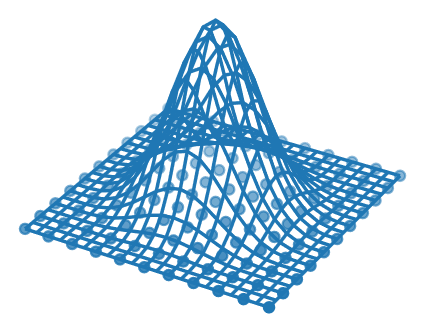
\includegraphics[scale=0.8]{SPH_Kernel-3D.png} \\
  		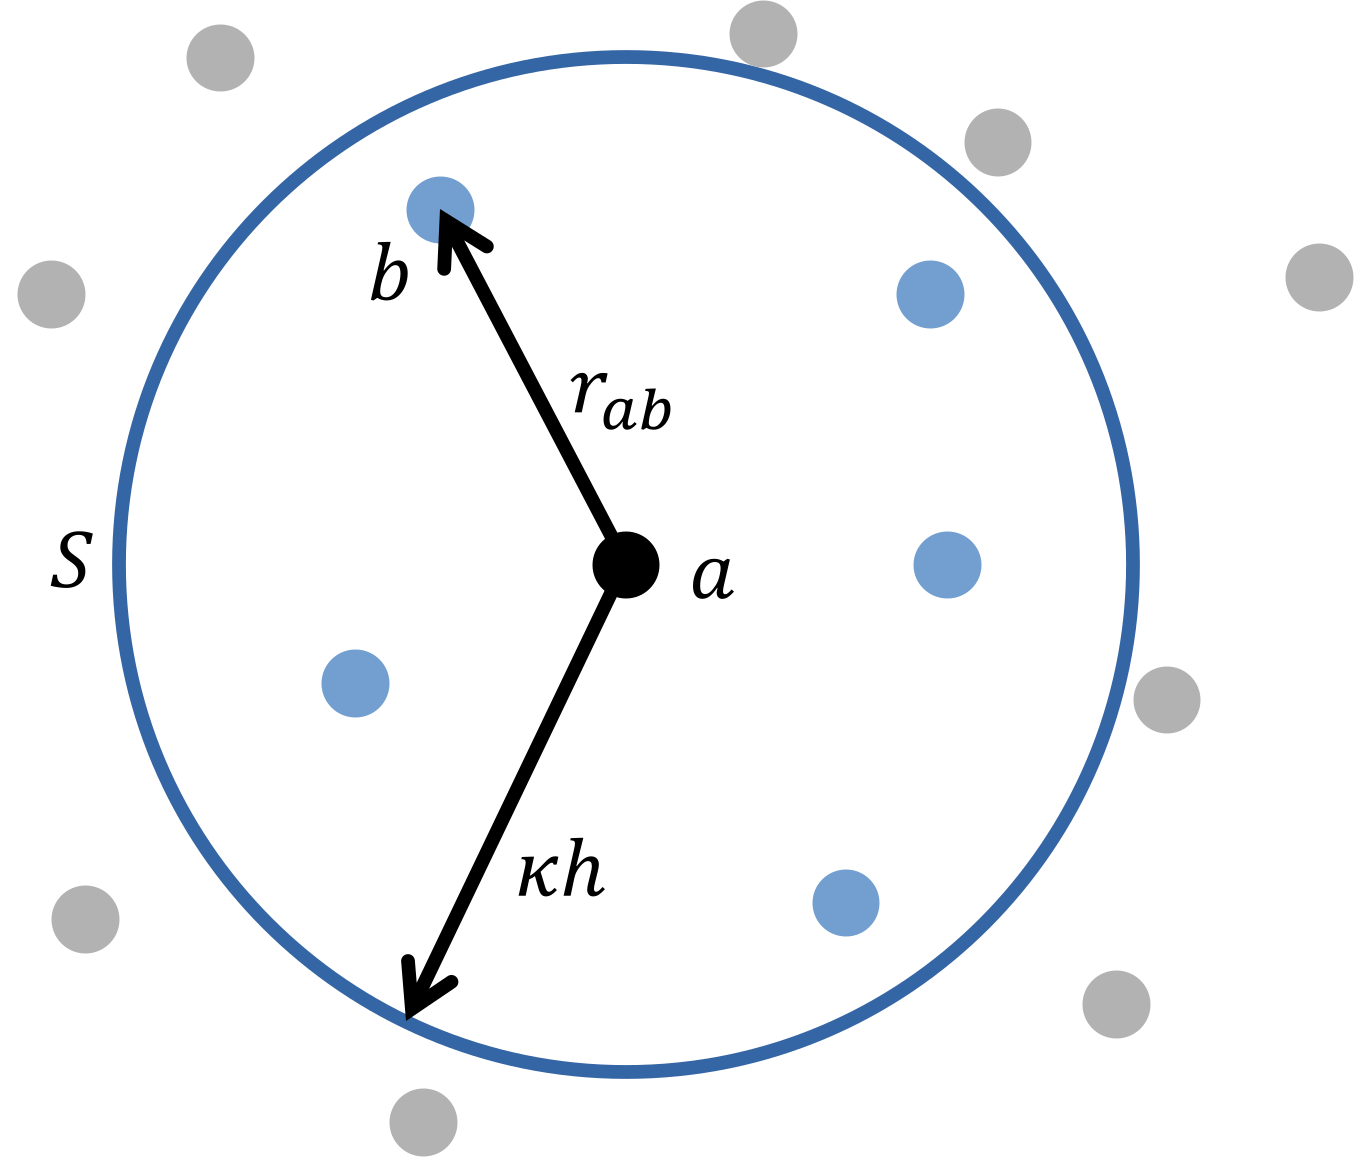
\includegraphics[scale=0.8]{SPH_Kernel-2D.png} 
  		\caption{Representation of a smoothing function used for the representation of a physical quantity in SPH.}
  		\label{fig:Kernels-SPH}
  	\end{figure}
  \end{column}
  \end{columns}
  \end{block}
  
	\vspace{0.79cm}
	
  \begin{block}{\textbf{3. Validation of our numerical model}}
  \begin{columns}
  \begin{column}{0.34\textwidth}\rightskip=0pt\leftskip=0pt
  We first focus on the thermal behavior of a 2D cryolava box at rest in contact with Methane Clathrate Hydrates substrate, compare it to the results of \emph{Davies et al (2010)} \cite{Davies2010} and find a strong agreement with the latter.
  
  \begin{figure}[h]
  	\caption{Heat loss per unit area from a flow or impact melt upper surface as a function of surface temperature and process
of heat removal. Adapted from \emph{Davies et al 2010}}
  \end{figure}
  \end{column}
  \begin{column}{0.62\textwidth}
  The next step is to study the rheological behavior of the cryolava.
  \begin{figure}[!h]
  	\centering
  	\includegraphics[scale=1.3]{../../Codes/pySPH_perso/2022-08-22-Cuve/HeatLoss.pdf} 
  \end{figure}
  \end{column}
  \end{columns}
  \end{block}
  
  \end{column}

\begin{column}{.495\linewidth}
 
 
  \begin{block}{\textbf{4. Rheology of terrestrial lavas}}
  \rightskip=0pt\leftskip=0pt
  \begin{columns}
  \begin{column}{0.49\textwidth}\rightskip=0pt\leftskip=0pt
  Several rheological models exist to describe lava flows (fig. \ref{fig:ModelsDescription}):
  \begin{itemize}
  	\item A newtonian fluid (example: water);
  	\item A non-newtonian fluid:
  	\begin{itemize}
  		\item A Bingham fluid (example: paint);
  		\item A power-law fluid (example: suspensions)
  		\item A Herschel-Bulkley (HB) fluid (more general; see eq. \eqref{eq:HBmodel}).
  	\end{itemize}
  \end{itemize}
  Terrestrial lavas contain mainly silicates and are studied in the context of risk estimation for human infrastructures.
  
  We can relate the shear stress of a fluid $\tau$ as function of its shear rate $\dot \gamma$:
  
  \begin{equation}
  	\tau \sim \eta_{app} \dot \gamma
  \end{equation}
  
  	The HB model is as followed:
  	\begin{equation}
  		\eta_{app} = \eta \dot \gamma^{n-1} + \frac{\tau_y}{\dot \gamma}\left(1-e^{-m \dot \gamma}\right)
  		\label{eq:HBmodel}
  	\end{equation}
  	with $n$ and $m$: parameters.
  \end{column}
  \begin{column}{0.49\textwidth}
  	But then, what will be the rheology of cryolava on Titan ?\vspace{-1cm}
  	\begin{figure}[h]
  		\centering
  		\includegraphics[scale=1.2]{Python_Figures/ShearStress_ShearRate.pdf} 
  		\caption{Description of different fluid flows, for Newtonian, Bingham, and several HB rheologies, $n=1$.}
  		\label{fig:ModelsDescription}
  	\end{figure}
  	%Cryolava Titan ?
  \end{column}
  \end{columns}\vspace{5pt}
  
  	Example with  $n=1$:
  	$m\rightarrow \infty \Rightarrow$ Bingham;
  	$m=0\Rightarrow$ Newton
  \end{block}
  
  \vspace{0.5cm}
  
  \begin{block}{\textbf{5. Description of cryolava -- Impact on rheology}}
  \rightskip=0pt\leftskip=0pt  
  The composition of cryolavas can affect their behavior, then it is important to understand their composition. If we assume that Titan's cryolavas are composed mostly of water, with a concentration $C$ of ammonia between 16\% and 32\% (weight), therefore, according to laboratory experiments \cite{kargel_1990}, the rheological behavior is:
  \begin{equation*}
  	\left\{
  	\begin{matrix}
  		\mathsf{Newtonian} & \mathsf{,\ if}\ C> 29\% \\
  		\mathsf{non-Newtonian} &\mathsf{,\ if}\  C \leq 29\% 
  	\end{matrix}
  	\right.
  \end{equation*}
  
  In addition, the addition of even 1\% methanol to the contents could totally change the rheology and therefore the behavior of the cryolava.
  
  
  

  
  \end{block}
  
    \vspace{0.5cm}
  \begin{block}{\textbf{6. Derivation of cryolava rheology from observations}} \rightskip=0pt\leftskip=0pt
  
  It is possible to deduce the rheological characteristics of a lava, and in particular the shear rate, from the observation of its flows. For a Bingham fluid, we can find its magnitude with this simple approach \cite{hulme_1974}:\vspace{-1cm}
  \begin{columns}
  \begin{column}{0.49\textwidth}\rightskip=0pt\leftskip=0pt
  \begin{equation}
  	\tau_y = \frac{\rho g h^2}{w}
  \end{equation}
  with $\tau_y$ the yield strength, $\rho$ the density, $g$ the acceleration of gravity, $h$ the height of the levee, $w$ the width of the levee. \emph{Lopes et al (2007)} \cite{Lopes2007} found with this technique an effective viscosity of $\sim 10^4\ Pa\ s$ for a flow emanating from a bright-rimmed circular feature ($41^\circ W$, $47^\circ N$) .
  
  The work of \emph{Kargel (1991)} \cite{kargel_1990} gives us an effective viscosity of $\sim 10^1\ Pa\ s$ for $\{H_2O;NH_3\}$ mixtures, and $\sim 10^4\ Pa\ s$ for $\{H_2O;NH_3;CH_3OH\}$ mixtures.
  \end{column}
  \begin{column}{0.49\textwidth}
  	\begin{figure}[h]
  	\centering
  	\includegraphics[scale=0.85]{levee.png} 
  	\caption{Schematic representation of a lava flow following
the model of \emph{Hulme (1974)} \cite{hulme_1974}. Adapted from \emph{Wadge and Lopes (1991)} \cite{WadgeLopes}.}%rajouter de quelle coulee de lave est appoliqué le resultat, puis qu'on favorise le dernier melange
  	\end{figure}
  	Therefore, we can consider the cryolava flow as a $\{H_2O;NH_3;CH_3OH\}$ mixture.
  \end{column}
  \end{columns}

  \end{block}
  
  
   \end{column}
   


  
  %%%%%%%%%%%%%%%%%%%%%%%%%%%%%%%%%%%%%%%%%%%%%%%%%%%%%%%%%%%

  \end{columns}
  
  \vspace{1cm}
  
\begin{block}{\textbf{Conclusion and future work}}\rightskip=0pt\leftskip=0pt
%validation de la methode sph-comportement thermique/ estimation grossiere des parametres rheologiques de la cryolave titanienne
%passer de la lave au repos à un ecoulement non-newtonien en refroidissement + comparer avec les observations
% Our work is particularly relevant in the perspective of the Dragonfly mission which will explore the region of the Selk crater, where solidified cryolava may be expected
	\textbf{We have confirmed the relevance of the SPH method for the thermal simulation of the cryolava, and obtained an estimate of its rheological parameters. In future works, we will simulate cooling non-Newtonian flows and compare the results obtained with observations. This work is greatly relevant in the perspective of the Dragonfly mission \cite{Dragonfly}, which will explore the Selk crater region and where solidified cryolava may be expected.}
\end{block}

    \vspace{1cm}

\begin{block}{\textbf{References}}\rightskip=0pt\leftskip=0pt
	\begin{columns}
	\begin{thebibliography}{9}
		\begin{column}{0.3\textwidth}\vspace{-1.5cm}
		\bibitem{nixon}
		{\textsc{Nixon}, C. A., et al. \emph{Planetary and Space Science} 155 (2018): 50-72.}
		\bibitem{Neish}
		{\textsc{Hedgepeth}, Joshua E., et al. \emph{Icarus} 344 (2020): 113664.}
		\bibitem{GingoldMonaghan}
		{\textsc{Gingold}, Robert A., and Joseph J. \textsc{Monaghan}. \emph{MNRAS} 181.3 (1977): 375-389.}
		\bibitem{Davies2010}
		{\textsc{Davies}, Ashley Gerard, et al. \emph{Icarus} 208.2 (2010): 887-895.}
		\end{column}
		\begin{column}{0.31\textwidth}\vspace{-1.5cm}
		\bibitem{Lopes2013}
		{\textsc{Lopes}, Rosaly MC, et al. \emph{J. Geophys. Res.: Planets} 118.3 (2013): 416-435.}
		\bibitem{kargel_1990}
		{\textsc{Kargel}, J. S., et al. \emph{Icarus} 89.1 (1991): 93-112.}
		\bibitem{hulme_1974}
		{\textsc{Hulme}, G. \emph{Geophysical Journal International} 39.2 (1974): 361-383.}
		\end{column}
		\begin{column}{0.32\textwidth}\vspace{-1.5cm}
		\bibitem{Lopes2007}
		{\textsc{Lopes}, Rosaly MC, et al. \emph{Icarus} 186.2 (2007): 395-412.}
		\bibitem{WadgeLopes}
		{\textsc{Wadge}, G., and R. M. C. \textsc{Lopes}. \emph{Bulletin of Volcanology} 54.1 (1991): 10-24.}
		\bibitem{Dragonfly}
		{\textsc{Lorenz}, Ralph D., et al. \emph{The Planetary Science Journal} 2.1 (2021): 24.}
		\end{column}
	\end{thebibliography}
	\end{columns}
\end{block}
    
\end{frame}

\end{document}
